\documentclass[ignorenonframetext,]{beamer}

\setbeamertemplate{caption}[numbered]
\setbeamertemplate{caption label separator}{: }
\setbeamercolor{caption name}{fg=normal text.fg}

\beamertemplatenavigationsymbolsempty
\usepackage{lmodern}
\usepackage{amssymb,amsmath}
\usepackage{ifxetex,ifluatex}
\usepackage{fixltx2e} % provides \textsubscript
\ifnum 0\ifxetex 1\fi\ifluatex 1\fi=0 % if pdftex
  \usepackage[T1]{fontenc}
  \usepackage[utf8]{inputenc}
\else % if luatex or xelatex
  \ifxetex
    \usepackage{mathspec}
  \else
    \usepackage{fontspec}
  \fi
  \defaultfontfeatures{Ligatures=TeX,Scale=MatchLowercase}
\fi

% Start adding some content
\usepackage{graphicx}
\usepackage{color}
\usepackage{beamerthemebars}
\usepackage{multicol}
\usepackage{multirow}
\usepackage{hyperref}


\usetheme{Frankfurt}
%%redefined colors for beamer
%\definecolor{beamer@UIUCblue}{RGB}{0,60,125}
%\definecolor{beamer@UIUCorange}{RGB}{244,127,36}
%% taken from
%% http://identitystandards.illinois.edu/graphicstandardsmanual/generalguidelines/colors.html
%
%\definecolor{beamer@UIUCgray}{RGB}{210,210,210}
%\definecolor{beamer@UIUCgray2}{RGB}{244,244,244}
%
%\setbeamercolor{frametitle}{fg=beamer@UIUCblue,bg=beamer@UIUCgray}
%\setbeamercolor{normal text}{fg=black}
%\setbeamercolor{title}{fg=beamer@UIUCblue,bg=beamer@UIUCorange}
%\setbeamercolor{item projected}{fg=white,bg=beamer@UIUCorange}
%
%% Boxes
%\setbeamercolor{block title}{fg=beamer@UIUCblue,bg=beamer@UIUCorange}
%\setbeamercolor{block body}{fg=blue,bg=beamer@UIUCblue!80}
%\setbeamercolor{title in head/foot}{fg=beamer@UIUCblue,bg=beamer@UIUCgray}
%\setbeamercolor{author in head/foot}{fg=white,bg=beamer@UIUCblue}
%\setbeamercolor{institute in head/foot}{fg=white,bg=beamer@UIUCorange}
%\setbeamercolor{date in head/foot}{fg=white,bg=beamer@UIUCorange}
%\setbeamercolor{section in head/foot}{fg=white,bg=beamer@UIUCblue}
%\setbeamercolor{subsection in head/foot}{fg=white,bg=beamer@UIUCorange}
%
%
%\hypersetup{colorlinks=true,urlcolor=beamer@UIUCblue,linkcolor=beamer@UIUCblue,% link color controls section, subsection, and title
%citecolor = beamer@UIUCorange,
%anchorcolor = beamer@UIUCorange}
%
%%override title link color
%\addtobeamertemplate{headline}{\hypersetup{linkcolor=.}}{}
%\addtobeamertemplate{footline}{\hypersetup{linkcolor=.}}{}
%
%% Setup blocks
%\setbeamercolor{block title}{fg = white, bg = beamer@UIUCblue}
%\setbeamercolor{block body}{fg=black,bg=beamer@UIUCgray2}
%
%\setbeamercolor{block title alerted}{fg = white, bg = beamer@UIUCorange}
%\setbeamercolor{block body alerted}{fg=black,bg=beamer@UIUCgray2}
%
%\setbeamercolor{block title example}{fg = beamer@UIUCblue, bg = beamer@UIUCgray}
%\setbeamercolor{block body example}{fg=black,bg=beamer@UIUCgray2}

% use upquote if available, for straight quotes in verbatim environments
\IfFileExists{upquote.sty}{\usepackage{upquote}}{}
% use microtype if available
\IfFileExists{microtype.sty}{%
\usepackage{microtype}
\UseMicrotypeSet[protrusion]{basicmath} % disable protrusion for tt fonts
}{}
\newif\ifbibliography
\usepackage{graphicx,grffile}
\makeatletter
\def\maxwidth{\ifdim\Gin@nat@width>\linewidth\linewidth\else\Gin@nat@width\fi}
\def\maxheight{\ifdim\Gin@nat@height>\textheight0.8\textheight\else\Gin@nat@height\fi}
\makeatother
% Scale images if necessary, so that they will not overflow the page
% margins by default, and it is still possible to overwrite the defaults
% using explicit options in \includegraphics[width, height, ...]{}
\setkeys{Gin}{width=\maxwidth,height=\maxheight,keepaspectratio}

% Prevent slide breaks in the middle of a paragraph:
\widowpenalties 1 10000
\raggedbottom


\setlength{\parindent}{0pt}
\setlength{\parskip}{6pt plus 2pt minus 1pt}
\setlength{\emergencystretch}{3em}  % prevent overfull lines
\providecommand{\tightlist}{%
  \setlength{\itemsep}{0pt}\setlength{\parskip}{0pt}}
\setcounter{secnumdepth}{0}
\usepackage{amsmath, bbm}


\author[
Xuelong Wang
]{Xuelong Wang}
\date[
11/29/2017
]{
November 29, 2017
}

% Option to fake out the raw_tex plugin and, thus, enabling the embedding of
% markdown within a column scheme.
% See:
% (1) https://groups.google.com/forum/#!msg/pandoc-discuss/vcy7v9Uk95U/LDgWJTHTRR4J
% (2) http://stackoverflow.com/questions/15142134/slides-with-columns-in-pandoc
\def\begincols{\begin{columns}}
\def\endcols{\end{columns}}

\begin{document}

% Necessary due to the ignorenonframetext requirement
% See: http://tex.stackexchange.com/questions/181032/ignorenonframetext-option-breaks-frame-background-color-option
\mode<all>{
\title[
PCA on Big Data
]{
%\begin{columns}
%\column{.25\textwidth}
%\hspace{.2in}
%\vspace{.1in}
%\includegraphics{ilogo.pdf}
%\column{.85\textwidth}
Big Data Dimension Reduction using PCA
%\end{columns}
}
}
\mode*

\frame{\titlepage}

\begin{frame}
\tableofcontents[hideallsubsections]
\end{frame}

\section{Introduction}\label{introduction}

\subsection{Introduction}\label{introduction-1}

\begin{frame}{Challenge of Big Data}

\begin{enumerate}
\def\labelenumi{\arabic{enumi}.}
\tightlist
\item
  Memory Barrier\\
\end{enumerate}

\begin{itemize}
\tightlist
\item
  The size of data is too large to load into memory
\item
  More specifically, n is way more large than p
\end{itemize}

\begin{enumerate}
\def\labelenumi{\arabic{enumi}.}
\setcounter{enumi}{1}
\tightlist
\item
  The computation time\\
\end{enumerate}

\begin{itemize}
\tightlist
\item
  It could be very time consuming if only use single core or cluster
\end{itemize}

\end{frame}

\begin{frame}{Solution}

\begin{enumerate}
\def\labelenumi{\arabic{enumi}.}
\tightlist
\item
  Sufficient statistics
\end{enumerate}

\begin{itemize}
\tightlist
\item
  PCA regression only uses sufficient statistics
\item
  Sufficient statistics can be calculated by scanning the data
  row-by-row
\end{itemize}

\begin{enumerate}
\def\labelenumi{\arabic{enumi}.}
\setcounter{enumi}{1}
\tightlist
\item
  Parallel computation\\
\end{enumerate}

\begin{itemize}
\tightlist
\item
  Multiple threads
\item
  Map-Reduced structure
\end{itemize}

\end{frame}

\section{PCA Regression}\label{pca-regression}

\subsection{Classical PCA}\label{classical-pca}

\begin{frame}{Basic idea of PCA}

\begin{block}{Singular Value Decomposition}

\begin{gather*} 
  X_s = UDV^T \text{~~,where~~~} x_{ij,s} = \frac{x_{ij} - \bar{x}}{s_j} \\
  U = (u_1, \dots, u_r) \text {~is a n by r orthogonal matrix~} \\
  D = diag(d_1, \dots, d_r) \text {~is a r by r diagonal matrix~} \\
  V = (v_1, \dots, v_r) \text {~is a p by r orthogonal matrix~} \\
\end{gather*}

\end{block}

\end{frame}

\begin{frame}{Basic idea of PCA}

\begin{block}{Principle Component and Loading}

\begin{align*} 
  X_s &= \underbrace{\begin{bmatrix} d_1u_1 \hdots  d_ru_r \end{bmatrix} }_\text{PCs}
         \underbrace{\begin{bmatrix} v_1^T \\
                         \vdots \\
                         v_r^T \\
         \end{bmatrix}}_\text{Loading}
\end{align*}

\begin{itemize}
\tightlist
\item
  \(PC_j = d_j\pmb{u_j} = X\pmb{v_j}\) is the jth principle component
\item
  The sample variance of \(PC_j\) is \(d_j^2/n\)
\end{itemize}

\end{block}

\end{frame}

\begin{frame}{Basic idea of PCA}

\begin{block}{Reduced matrix $X_{s,k}$}
\begin{align*}
  X_{s,k} &= \sum_{j=1}^{k}d_j\pmb{u_jv_k} = U_kD_kV_k^T, \text{~~Its Variation ~}  \sum_{j=1}^kd_j^2/n. 
\end{align*}
\end{block}

Its proportion of the total variation is

\[
\lambda_k = \frac{\sum_{j=1}^{k}d_j^2}{\sum_{j=1}^{r}d_j^2} 
\]

\begin{itemize}
\tightlist
\item
  If a small k such that \(\lambda_k \approx 1\), we can use \(U_kD_k\)
  in the follow up analysis
\end{itemize}

\end{frame}

\begin{frame}{Follow-up analysis}

The PCA approach is applied to a linear regression

\begin{block}{Model}

\[
  y = \mathbbm{1}_{n}\alpha_s + U_kD_K\beta_{s,k} + \epsilon_{s,k},
\]

Where \(\epsilon_{s,k} \sim N(0, \sigma^2_{s,k}\pmb{I}_n)\)

\end{block}

\begin{block}{LSE and their variance}

\[
  \hat{\alpha}_s = \bar{Y},~~ \hat{\beta}_{s,k} = D_k^{-1}U_k^Ty  ~~\textcolor{red}{(PCs~are~ Orthogonal)}
\]

\[
  \mathbb{V}(\hat{\sigma}_{s,k}^2) = [y^T(\underbrace{\mathbb{I}_n - \mathbb{J}_n/n - U_kU_k^T}_{\mathbb{I}_n - P_k})y]/(n-k)
\]

\end{block}

\end{frame}

\section{Sufficient Statistics}\label{sufficient-statistics}

\subsection{Def}\label{def}

\begin{frame}{Sufficient Statistics}

\begin{block}{Factorization Theorem}
\[
  f(x_1, x_2, ... , x_n;\theta) =\phi\left[u(x_1, ... , x_n);\theta \right] h(x_1, ... , x_n)
\]

\end{block}

\begin{itemize}
\tightlist
\item
  \(u(x_1, ... , x_n)\) is the sufficient statistics for \(\theta\)
\item
  If \(\theta\) is a vector, then \(u(x_1, ... , x_n)\), the Joint
  Sufficient Statistics, will be also a vector.
\end{itemize}

\end{frame}

\begin{frame}{Sufficient Statistics}

\begin{block}{model}
\[
  y = \mathbbm{1}_{n}\alpha + X\beta + \epsilon,~\epsilon \sim N(0, \sigma^2\pmb{I}_n)
\]
\end{block}

\begin{block}{Log-Likelihood function}

\begin{multline*}
  \log{\{f(y|x, \alpha, \beta, \sigma)\}} =  \frac{n}{2}\log{2\pi} - \frac{n}{2}\log{\sigma^2} \\ -\frac{1}{2\sigma^2}(c_{yy} - 2\alpha c_y + 2c_{xy}\beta + n\alpha^2 + 2\alpha c_x^T\beta +\beta^T C_{xx} \beta) 
\end{multline*}

\end{block}

\begin{itemize}
\item
  Define:
  \(\mathcal{C}(y, X) = (c_0, c_{yy}, c_y, \pmb{c}_{xy}, \pmb{c}_x, C_{xx})\)
\item
  Note that \(\ell(\alpha, \beta, \sigma)\) only depends on
  \(\mathcal{C}(y, X)\)
\end{itemize}

\end{frame}

\subsection{Sufficient statistics for
PCA}\label{sufficient-statistics-for-pca}

\begin{frame}{More about \(\mathcal{C}(y, X)\)}

\begin{block}{Elements of $\mathcal{C}(y, X)$}
  \begin{gather*}
  c_{0} = n, ~c_{yy} = \sum_{i=1}^n Y_i^2, ~c_y = \sum_{i=1}^n Y_i, \\
  ~c_{xy} =\sum_{i=1}^n Y_ix_i,~c_x = \sum_{i=1}^n x_i, ~C_{xx} = \sum_{i=1}^n x_ix_i^T
  \end{gather*}
\end{block}

\begin{itemize}
\tightlist
\item
  Notice that \(\mathcal{C}(y, X)\) is the Joint sufficient statistics
  for \((\alpha, \beta, \sigma)\)
\item
  All terms are in the summation format, so it can be calculated by
  reading the data row-by-row
\end{itemize}

\end{frame}

\begin{frame}{Computation of \(\mathcal{C}(y, X)\)}

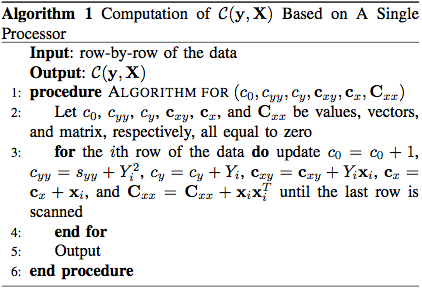
\includegraphics[width=0.7\linewidth]{./Alg_1}

\begin{itemize}
\tightlist
\item
  \(\mathcal{O}((p+1)^2)\) memory size\\
\item
  \(\mathcal{O}(n(p+1)^2)\) floating operations
\end{itemize}

\end{frame}

\begin{frame}{Sufficient Statistics based on \(X_s\)}

\begin{block}{Statistics affected by standardization}
\[
  C_{s, xx} = X^T_{s}X_{s},~~ c_{s,xy} = X_s^Ty, ~~~c_{s, x} = \mathbbm{1}_{n}^TX_s/n
\]
\end{block}

\begin{itemize}
\tightlist
\item
  It can be proved that, those statistics can be computed directly from
  \(\mathcal{C}(y, X)\)
\end{itemize}

\begin{block}{Key step}
\[
c_{s,k,xy} = V_k^Tc_{s,xy} = V_k^TVDU^Ty= D_kU_k^Ty ~\Rightarrow ~U_k^Ty = D^{-1}_kc_{s,k,xy}    
\]
\end{block}

\end{frame}

\section{PCA on Big Data}\label{pca-on-big-data}

\subsection{}\label{section}

\begin{frame}{Back to PCA regression}

\[
  X_s = UDV^T
\]

Since n is large, it's not available to calculate U. However, we can
only use \(V\) and \(D\) to get the estimated coefficients and variance.

\begin{block}{PCA regression based on sufficient statistics}

\begin{enumerate}
\def\labelenumi{\arabic{enumi}.}
\tightlist
\item
  \(D\), \(V\) can be calculated by \(C_{s, xx} = X_s^TX_s = VD^2V^T\)
\item
  \(U_k^Ty = D^{-1}_kc_{s,k,xy}\), so
  \(\hat{\beta}_{s,k} = D^{-2}_kc_{s,k,xy}\)
\item
  \(\mathbb{V}(\hat{\sigma}_{s,k}^2) = [c_{yy}-c_{yy}/n - c_{s,k,xy}^TD^{-2}_kc_{s,k,xy}]/(n-k)\)
\end{enumerate}

\end{block}

\end{frame}

\begin{frame}{Parallel Computation with Distributed Systems}

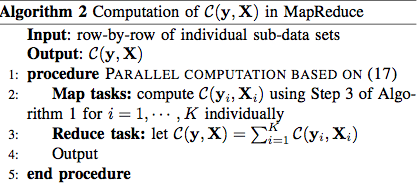
\includegraphics{./Alg_2.png}

\end{frame}

\begin{frame}{}

\begin{center}
\Huge Thank you
\end{center}

\end{frame}

\begin{frame}{Reference}

\hypertarget{refs}{}
\hypertarget{ref-ref5}{}
Tonglin Zhang, Baijian Yang. 2016. ``Big Data Dimension Reduction Using
Pca.''

\end{frame}

\end{document}
